% Motivation
The labor income share, its evolution and distributional implications, have been of interest for economists since at least the work of \citet{Kaldor1955Alternative}.\footnote{Starting with \citet{Blanchard1997Medium} a growing literature has documented changes in the labor share. A renewed interest in its distributional consequences is largely due to \citet{Atkinson2009Factor}, and it is a key determinant of the distribution of personal income; see \citet{Checchi2010Labour} and \citet{Bengtsson2018Capital}.}
While initially existing evidence indicated that it remained stable for decades, several OECD countries have witnessed a decline since the beginning of the 1970s and a heated debate has emerged trying to understand the reasons for these dynamics; see, for example, \citet{Karabarbounis2014Global} and \citet{Elsby2013Decline}. These countries also experienced significant changes in the age structure of their population following the birth of the so-called \textit{baby-boomer} cohorts---born between 1945 and 1965. 
Yet, the literature on the labor share has paid no attention to the coincidence in timing between, on the one hand, the start of the decline of the labor share, and on the other hand, the entry of this latter cohort into adulthood, i.e. entering into the labor market and reaching voting age.

% Empirical motivation
Figure \ref{chap1-fig:emp-lsdepcor} depicts the negative correlation between the old-age-dependency ratio---which is driven by the position in the life cycle of the boomer cohorts---and the labor share across several OECD countries between 1950 and 2019.\footnote{The old-age-dependency ratio is defined as the ratio of the number of individuals above 60 over the number of those between 20 and 60. When the boomers are young, they maintain the old-age-dependency ratio relatively low although their elders are aging due to the increasing life expectancy. Once they become old, the ratio explodes.}
% Empirical motivation
\begin{figure}[!tb]
	\centering
	\caption{Labor share and old-age-dependency ratio}\label{chap1-fig:emp-lsdepcor}
	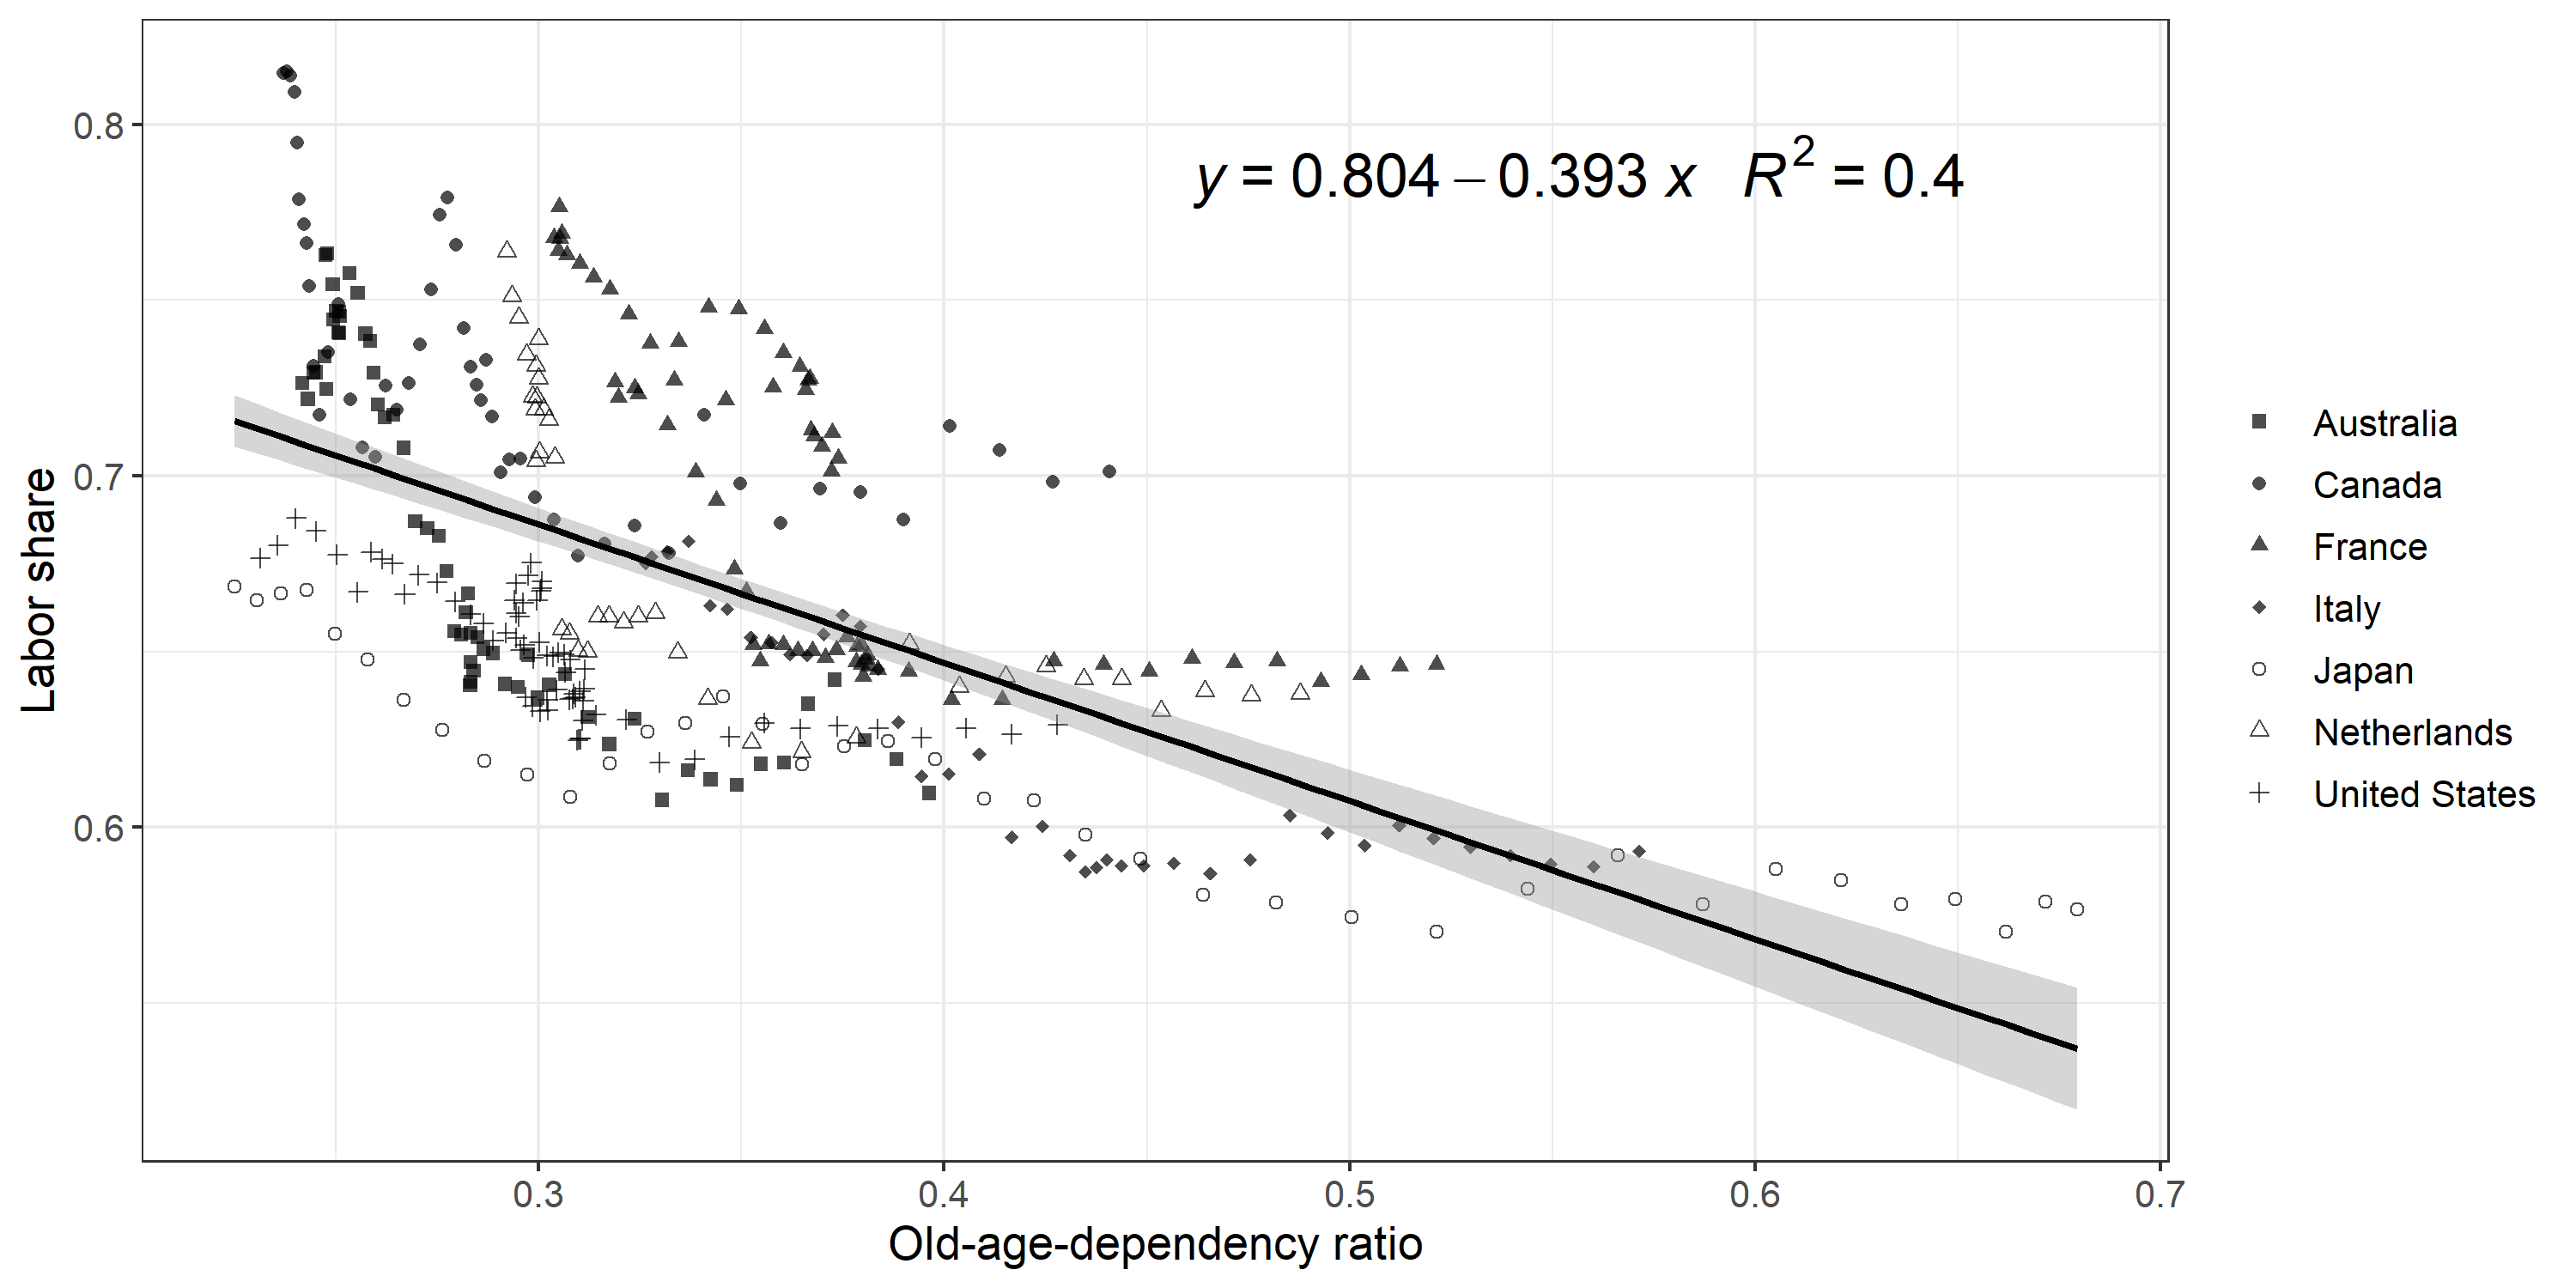
\includegraphics[width=\linewidth]{chap1/graphic/emp-lsdepcor.png}
	\vspace{-3em}
	\justify\singlespacing\footnotesize\textit{Notes:} The figure displays the negative correlation between the labor share and old-age-dependency ratio for several OECD countries. Labor share data are from the \href{https://www.rug.nl/ggdc/productivity/pwt/}{Penn World Table 10.0}. The old-age-dependency ratio is defined as the number of individuals above 60 over the number of those between 20 and 60. The ratio is computed with demographic data from the ``medium variant'' estimates from the \href{https://population.un.org/wpp/}{United Nations World Population Prospects 2017}.
\end{figure}
These data display a positive correlation, as the older the population the lower the labor share. 
Figure \ref{chap1-fig:emp-pubdepcor} shows cross-country correlations between the old-age-dependency ratio and the ratio between two public policy instruments, thus, providing empirical motivation also for linking public policy to the age structure of the population.\footnote{Looking also at the timing of labor market reforms---on employment protection legislation, public pension systems, non-employment benefits, and migration policies---in 14 OECD countries between 1986 and 2005, \citet{Pica2010Capital} shows that the number of reforms raising labor market flexibility has increased over time, hence, as the boomers' cohorts aged.}
\begin{figure}[!tb]
	\centering
	\caption{Public pension to unemployment spending ratio and old-age-dependency ratio}\label{chap1-fig:emp-pubdepcor}
	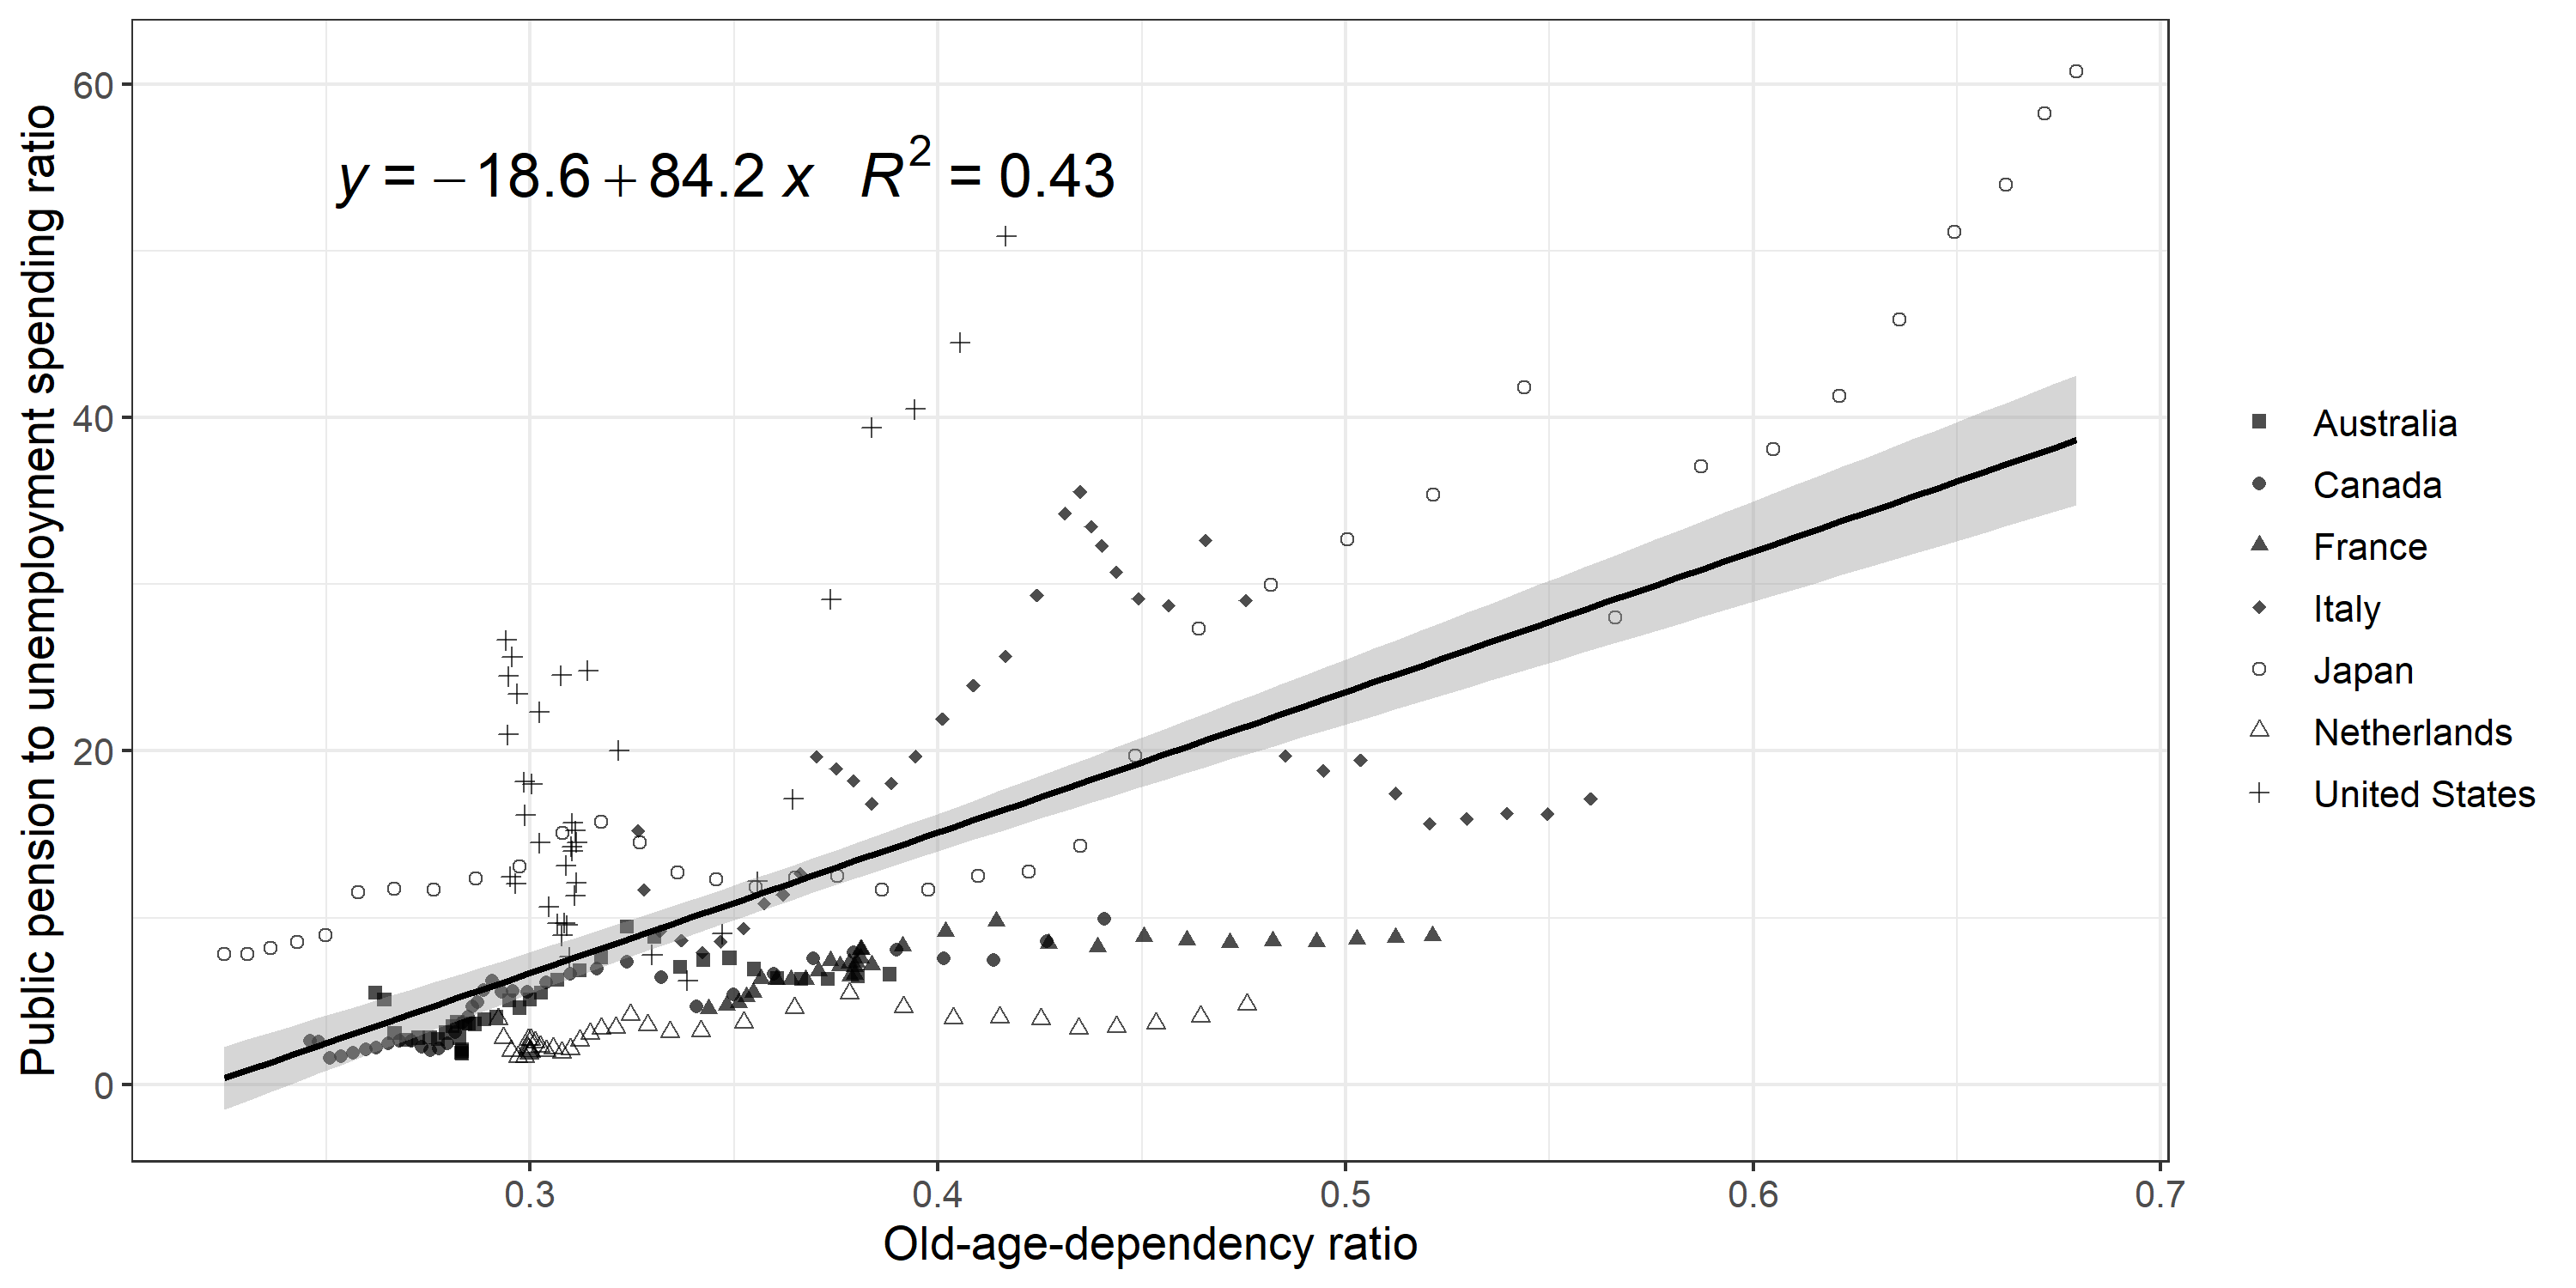
\includegraphics[width=\linewidth]{chap1/graphic/emp-pubdepcor.png}
	\vspace{-3em}
	\justify\singlespacing\footnotesize\textit{Notes:} The figure displays the positive correlation between the public pension to unemployment spending ratio and old-age-dependency ratio for several OECD countries. The public pension to unemployment spending ratio is computed using the total public unemployment spending and the total public pension spending (both as shares of GDP) from the OECD data. The old-age-dependency ratio is defined as the number of individuals above 60 over the number of those between 20 and 60. The ratio is computed with demographic data from the ``medium variant'' estimates from the \href{https://population.un.org/wpp/}{United Nations World Population Prospects 2017}.
\end{figure}
An increase in the old-age dependency ratio is associated with an increase in public pensions as a share of GDP relative to the share of unemployment spending. These data indicate that as the boomer cohorts age, public policy shifts in favor of old-age specific government spending.

% In this paper
In this paper, I argue that the observed shift away from labor toward capital is a response to changes in labor market institutions endogenously determined by the age structure of the population, a novel mechanism that this paper is the first to identify. Through this new \textit{policy-mechanism} effect, boomers drove the decline of the labor share when they were young and continue to drive it down nowadays as they retire. 

My argument is based on the idea that the boomers drive public policy choices because the size of their cohort gives them large political weight. When they are young, they change labor market institutions in their favor which allows them to bargain greater wages. To thwart workers' appropriation of rents, firms shift away from labor toward capital which decreases the labor share. Once the boomers become old and retire, we would expect a reversal of the labor share dynamics as pro-worker labor market institutions dwindle which increases employment. However, the consequent positive effect of employment on the labor share is offset by the capital accumulation fostered by extensive savings of the boomers when they were young, implying a further decline.

%% What I do
% Describe model
I develop a two-period OLG model with young and old households. Both vote to determine public policy while they have different income sources and opposite objectives. Old agents receive capital income and favor old-age specific government spending, whereas the youth receive wages and support unemployment benefits as they face unemployment risk. As a large cohort of boomers arrives, they use their political weight---through voting---to raise taxes and unemployment benefits. Both latter increase the outside option of workers in wage bargaining which allows them to bargain greater wages. The representative firm shifts away from labor toward capital. When labor and capital are gross substitutes, this leads to the decline of the labor share. Once the boomers retire, the political weight of the young declines and so does the unemployment benefit which fosters employment. However, the positive effect of employment on the labor share is offset by capital accumulation due to the extensive savings of young boomers which have been fostered by their higher bargained wages.

% Two mechanism
My framework suggests that demographic dynamics affect the labor share in two different ways. On the one hand, there is a direct \textit{factor-accumulation} effect operating through the labor supply and capital stock. A large generation expecting to live longer, such as the boomers, results in a higher labor supply when they are young and a larger capital stock---fostered by their savings---once they retire. On the other hand, there is an indirect \textit{policy-mechanism} effect reflecting the inter-generational conflict over public policy. A large generation has relatively more political weight---with respect to their elders and their youngsters---which allows it to shape the public budget allocation in its favor through voting.

% Consequences on the labor market
Both effects have consequences for the wage bargaining taking place in the labor market. The factor-accumulation effect encompasses two dynamics: a larger capital stock allows firms to substitute labor with capital which increases the capital-to-labor ratio; while a greater labor supply decreases wages which fosters employment, hence reducing the capital-to-labor ratio. Conversely, the consequence of the policy-mechanism effect is straightforward. When the political weight of the youth increases, so do unemployment benefits which raise workers' outside option. Workers bargain greater wages which undermines employment as firms substitute labor with capital, hence, raising the capital-to-labor ratio. The framework provides dynamics of the capital-per-worker with respect to demographic dynamics that \textit{do not depend on} the elasticity of substitution between capital and labor.

% Elasticity of substitution
The elasticity of substitution between capital and labor plays a crucial role in the model as it determines whether an increase in capital per worker raises or reduces the labor share. To calibrate the model, I estimate this elasticity, respectively, for France and the United States, and find, respectively, the values 1.21 and 1.27.\footnote{
I follow the specification of \citet{Klump2007Factor}, I estimate a single-equation estimation from the two first-order conditions of the profit maximization for a CES production function with biased technical change. Periods of the estimate correspond to 1950-2018 for France and 1950-2019 for the US. See section \ref{chap1-calibration} for the details.} 
Both elasticities being greater than one imply that capital and labor are gross substitutes. Thus, any increase of the capital per worker decreases the labor share, which corresponds to the stylized facts for several OECD countries (\citealt{Karabarbounis2014Global}). There is a substantive debate about the value of this elasticity in the literature. For the United States, many studies tend to find an elasticity between 0.4 and 0.6 (\citealt{Antras2004Aggregate}, \citealt{Chirinko2008Sigma}, \citealt{LeonLedesma2010Identifying}, i.a.). Nonetheless, \citet{Chirinko2017Substitution} recently show that this elasticity is much greater than one when considering income shares defined net of depreciation, which is in line with my theoretical framework. \citet{Rognlie2016Deciphering} also argues that accounting for depreciation is more relevant when dealing with income distribution issues. My estimate builds on the two latter arguments and supports recent estimates considered in the labor share literature.\footnote{
\citet{Caballero1998Jobless} use a capital-labor elasticity of substitution about 6 to simulate French data. \citet{Karabarbounis2014Global} use cross-sectional data on 50 countries between 1975 and 2012 to find a baseline estimate of the elasticity about 1.28. \citet{Piketty2015About} shows that the capital-income ratio and capital share tend to be positively correlated, thus, arguing that only an elasticity above one can reconcile this stylized fact with the one-sector standard model.}

% Quantitative analysis
I calibrate the model for France and the US starting in 1950. The model replicates labor share dynamics until the 2010s, along with those of the labor market. It also provides predictions of future dynamics. In France, the labor share is predicted to steadily decline from 64.7\% in 2020 to 60.4\% by 2100; while in the US, it is predicted to remain stable at 62.7\% until 2040 before declining to 58.8\% by 2100. From 2020 onward and until the end of the century, on average, about one percentage point of the labor income share will shift to capital income every 20 years.

% Counterfactual and decomposition
Counterfactual analysis shows that the policy-mechanism effect is as important as the factor-accumulation effect. In fact, the former partially offsets the latter effect when the boomers are young, hence, reducing the labor share. Once they retire, this newly-identified effect dominates. This pattern holds for both countries.

% Who are the winners
Lastly, I conclude by showing that boomers are the winners of the age-related conflict despite the decline of the labor share when they are young. They manage to compensate their labor income losses through redistribution due to their political weight. Thus, boomer cohorts have been better off in terms of income with respect to their elders and their youngsters.

%% Contributions
% 1/ Consequences of changes in the age structure of the population
My paper is related to several strands of the literature. First, I contribute to the growing literature on the consequences of demographic changes for the allocation between capital and labor income. 
\citet{Schmidt2013Demographic} show that an aging population leads to more savings, hence, more capital. When capital and labor are gross
substitutes, the accumulation of capital shrinks the labor share. 
I build on their mechanism--- which I define as the direct factor-accumulation effect---and introduce a new mechanism, namely, the indirect policy-mechanism effect. %, suggesting that labor market institutions are endogenous to these population dynamics.
\citet{Albis2021Demographic} empirically find that an exogenous change in the net population growth rate leads to a decline of the labor share; while an exogenous change in the net migration rate increases the labor share.
My paper provides a theoretical framework that can explain both patterns through the lens of the factor-accumulation and policy-mechanism effects.
Recent work has focused on changes in the labor share across industries. Notably, \citet{Acemoglu2022Demographics} argue that firms decide to rely more on automation technologies to replace middle-aged workers in manual production tasks as the latter become scarce due to population aging. They predict that the labor share should decline in industries that are intensive in those tasks.
My work provides an additional mechanism that relates firms' response to constraints in optimizing production factors owing to endogenous changes in labor market institutions fostered by demographic dynamics.

% 2/ Labor share determinants
Second, my work is related to the literature on the determinants of the labor share. These determinants have been widely studied and debated, ranging from globalization (\citealt{Jayadev2007Capital}, \citealt{Pica2010Capital}, \citealt{Young2018Globalization}, \citealt{Autor2020Fall}, i.a.) to capital-biased technical change (\citealt{Acemoglu2002Directed},  \citealt{Acemoglu2003Labor}, \citealt{Karabarbounis2014Global}, i.a.) and labor market institutions (\citealt{Blanchard1997Medium}, \citealt{Bentolila2003Explaining}, \citealt{Bental2010Declining}, i.a.). \citet{Caballero1998Jobless} argue that pro-labor income institutions are a burden to firms because they limit their ability to optimize inputs but also because they enable workers to obtain a high income share. As a response, firms shift away from labor toward capital through biased technical change. My paper looks upstream of the key mechanism in \citet{Caballero1998Jobless} and reproduces it without the need for biased technical change; rather I endogenize changes in labor market institutions which are determined by the age structure of the population. I hence show that demography is a key determinant of the labor share and suggest that it can be at the root of several explanations that the literature has measured (see, for instance, \citealt{Bergholt2021Decline}).

% 3/ Role of demography in shaping institutions and macro consequences
Third, the paper fits into the literature on the role of demography in shaping institutions and its consequences for macroeconomic outcomes (\citealt{Lee2010Macroeconomic}, \citealt{Aksoy2019Demographic}). Prior work focuses on the optimal retirement age for economic growth (\citealt{Futagami2001Population}, \citealt{Gonzalez-Eiras2012Ageing}, i.a.) or the sustainability of pension systems (\citealt{DelaCroix2013Aging}, \citealt{Dedry2017Aging}, i.a.). I contribute to this literature by providing insights on a key macroeconomic indicator that has never been considered by this debate, namely, the allocation of income between capital and labor.

% 4/ Boomers
Lastly, I contribute to the scarce literature on the consequences of cohort dynamics for aggregate labor-market dynamics (\citealt{Shimer1998Why}, \citealt{Ferraro2020Aging}). My results suggest that the boomers' generations are important drivers of the declining labor share in France and the US, a concept that has so far not been put forward.

% Plan
This paper is organized as follows. Section \ref{chap1-theory} describes the model starting with households, then presenting the labor market and public policy, to analyze the equilibrium. Section \ref{chap1-quantitative} provides the quantitative analysis. I start with the data, before calibrating the model. I present model predictions, compare the factor-accumulation and policy-mechanism effects, and discuss who are the winners of the age-related conflict. Section \ref{chap1-conclusion} concludes.